%/*******************************************************************************
% * Copyright (c) 2009, A. Kaufmann and Elexis
% * All rights reserved. This program and the accompanying materials
% * are made available under the terms of the Eclipse Public License v1.0
% * which accompanies this distribution, and is available at
% * http://www.eclipse.org/legal/epl-v10.html
% *
% * Contributors:
% *    A. Kaufmann - initial implementation
% *    Patrick Chaubert und Tony Schaller, medshare GmbH - V2 enhancements
% *
% * $Id:$
% *******************************************************************************/

\documentclass[a4paper]{scrartcl}
\usepackage{german}
\usepackage[utf8]{inputenc}
\usepackage[german]{babel}
\usepackage[]{hyperref}
\usepackage{listings}
\usepackage{booktabs}
\usepackage[pdftex]{graphicx}

\lstset{extendedchars=false}

\title{Hilotec-Messwerte V2}
\author{medshare GmbH(V2), Antoine Kaufmann(V1)}

\begin{document}
\maketitle
\section{Einführung}
Dieses Elexis-Plugin ist dazu gedacht, Messungen und andere Erhebungsdaten in
Elexis strukturiert erfassen und verarbeiten zu können. Mit dem Plugin
\textit{hilotec-pluginstatistiken} wird es auch ermöglicht, Auswertungen
darüber zu erstellen, und die Werte als CSV zu exportieren.

Das Plugin stellt eine View "Hilotec Messwerte V2" zur Verfügung, die eine Übersicht über alle
Messungen eines Patienten bietet. Dort können auch neue Messungen erfasst und Bestehende bearbeitet (verändert oder gelöscht) werden.

Die Konfiguration der möglichen Messungen und deren Struktur wird in einer
XML-Datei spezifiziert.
\subsection{Neuerungen in V2}
In der V2 des Plugins sind zwei neue Datentypen hinzugekommen (datefield und counterfield). Zudem können bei numfield, calcfield und counterfield nun Zahlenformate und Rundungsmechanismen konfiguriert werden.


\section{Voraussetzungen}
\begin{itemize}
    \item Elexis ab V2.0
\end{itemize}

\section{Konfiguration}
Wie weiter oben bereits erwähnt, wird das Plugin über eine XML-Datei
konfiguriert. Diese Dateien befinden sich im Benutzerdatenverzeichnis von
Elexis:
\begin{description}
    \item[Windows:] \texttt{C:\textbackslash
                                Dokumente und Einstellungen\textbackslash
                                Benutzer\textbackslash Elexis\textbackslash
                                messwerte\_v2.xml}
    \item[Linux:] \texttt{/home/benutzer/elexis/messwerte\_v2.xml}
    % TODO: Mac?
\end{description}

Die verfügbaren Messungstypen werden mit \texttt{datatype}-Elementen im
Rootelement \texttt{datatypes} deklariert. Pro Messungstyp kann ein Name, der
intern (unter anderem auch für die IDataAccess-Schnittstelle und damit z.B. Nutzung der Messwerte als Platzhalter in Briefen) zur Identifikation
des Typs benutzt wird, dieser kann mit dem Attribut \texttt{name} festgelegt
werden. Die Messungsbezeichnung, die dem Benutzer angezeigt wird, kann über das
Attribut \texttt{title} konfiguriert werden. In der XML Datei sieht das
folgendermassen aus:
\begin{lstlisting}
<?xml version="1.0">
<datatypes>
  <datatype name="masse" title="Masse">
    <numfield name="gewicht" title="Gewicht" unit="kg" />
    <numfield name="groesse" title="Groesse" unit="m" />
  </datatype>
  <datatype name="bdruck" title="Blutdruck">
    <numfield name="bdsys" title="Systolisch" unit="mm Hg" />
    <numfield name="bddia" title="Diastolisch" unit="mm Hg" />
  </datatype>
</datatypes>
\end{lstlisting}

In den \texttt{datatype}-Tags können die zur Messung gehörenden Felder
eingetragen werden.

Bei allen Feldtypen sind die folgenden Attribute verfügbar:
\begin{description}
    \item[name:] Interner Feldname, muss eindeutig sein in dem Typ
    \item[title:] Dem Benutzer angezeigter Titel
    \item[unit:] Einheit (nur für den Benutzer)
\end{description}

Im Folgenden wird auf die einzelnen Feldtypen genauer eingegangen. Die
angegebenen Typnamen entsprechen gleichzeitig auch den XML-Tagnamen um Felder des
entsprechenden Typs zu generieren.


\subsection{strfield}
Ein- oder mehrzeiliges Textfeld
\begin{center}
    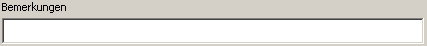
\includegraphics[width=12cm]{images/strfield.png}
\end{center}
\subsubsection{Attribute}
\begin{description}
    \item [default:] Standardwert, wenn die Messung neu erfasst wird
    \item [lines:] Anzahl Zeilen des Textfeldes \textit{[Standard: 1]}
\end{description}
\subsubsection{Beispiel}
\begin{lstlisting}
<strfield name="bemerk" title="Bemerkungen" lines="1" />
\end{lstlisting}


\subsection{numfield}
Zahlenfeld
\begin{center}
    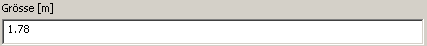
\includegraphics[width=12cm]{images/numfield.png}
\end{center}
\subsubsection{Attribute}
\begin{description}
    \item [default:] Standardwert, wenn die Messung neu erfasst wird
    \item [formatpattern:] Pattern für die Formatierung der angezeigten Zahl
    \textit{[Standard: \#0.\#]}
    \item [roundingmode:] Modus wie die angezeigte Zahl gerundet wird
    \textit{[Standard: HALF\_UP]}
\end{description}

\subsubsection{Beschreibung formatpattern Attribut}
Mit dem \texttt{formatpattern} Attribut kann angegeben werden wie die angezeigte Zahl
dargestellt werden soll. Die Formatierung wird beim Anzeigen angewendet. Es bassiert auf der Verwendung der JAVA Klasse
\textit{DecimalFormat}. Der Formatierungsstring kann eine Menge von
Formatierungsanweisungen vertragen (siehe Java API). Die beiden
wichtigsten Symbole sind \texttt{0} und \texttt{\#}. Beide repräsentieren
Ziffern. Weiter sind Punkt und Komma wichtig, welche als Dezimaltrenner und
zum Gruppieren der Ziffern dienen.
\begin{description}
  \item [0] Repräsentiert eine Ziffer – ist die Stelle nicht belegt, wird eine  Null angezeigt.
  \item [\#] Repräsentiert eine Ziffer – ist die Stelle nicht belegt, bleibt sie  leer, damit führende Nullen und unnötige Nullen hinter dem Komma nicht angezeigt werden.
  \item [.] Dezimaltrenner. Trennt Vor- und Nachkommastellen.
  \item [,] Gruppiert die Ziffern (eine Gruppe ist so groß wie der Abstand von
  "," zu "."). \\
  Wird für Tausendertrennzeichen verwendet.
\end{description}
\subsubsection{Beschreibung roundingmode Attribut}
Mit dem \texttt{roundingmode} Attribut kann angegeben werden, wie eine Zahl gerundet
werden soll. Die Rundung wird beim Speichern angewendet. Es basiert ebenfalls auf der Verwendung der JAVA Klasse
\textit{DecimalFormat} mit dem Enum \textit{RoundingMode}.
Folgende Auswahlmöglichkeiten stehen zur Verfügung:
\begin{description}
  \item [UP] Rundet die Zahl von 0 ausgehend auf
  \item [DOWN] Rundet die Zahl von 0 ausgehend ab
  \item [CEILING] Rundet die Zahl in positive Richtung auf
  \item [FLOOR] Rundet die Zahl in negative Richtung ab
  \item [HALF\_UP] Rundet die Zahl auf die nächste Ganzzahl, ab 0.5 wird aufgerundet \\
  (Standard-Einstellung und am häufigsten verwendete Rundungsregel)
  \item [HALF\_DOWN] Rundet die Zahl auf die nächste Ganzzahl, bei 0.5 wird
  abgerundet
  \item [HALF\_EVEN] Rundet die Zahl auf die nächste Ganzzahl, bei 0.5 wird immer
  auf die gerade Ganzzahl gerundet
\end{description}
\subsubsection{Beispiel}
\begin{lstlisting}
<numfield name="gewicht" title="Gewicht" unit="kg" formatpattern="0.00"
roundingmode="HALF_UP" />
\end{lstlisting}

\subsection{scalefield}
Feld um Ganzzahlen in einem eingegrenzten Bereich zu erfassen
\begin{center}
    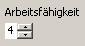
\includegraphics[width=2.3cm]{images/scalefield.png}
\end{center}
\subsubsection{Attribute}
\begin{description}
    \item[default:] Standardwert, wenn die Messung neu erfasst wird
    \item[min:] Kleinster erfassbarer Wert
    \item[max:] Grösster erfassbarer Wert
\end{description}
\subsubsection{Beispiel}
\begin{lstlisting}
<scalefield name="arfaeh" title="Arbeitsfaehigkeit"
  min="0" max="5" default="5" />
\end{lstlisting}

\subsection{enumfield}
Auswahlfeld mit einer fixen Liste an Auswahlmöglichkeiten
\begin{center}
    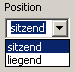
\includegraphics[width=2.2cm]{images/enumfield.png}
\end{center}
\subsubsection{Attribute}
\begin{description}
    \item[default:] Standardwert, wenn die Messung neu erfasst wird. Muss
                    angegeben werden und dem Wert einer Option aus der Liste
                    entsprechen.
\end{description}
\subsubsection{Unterelemente}
Die einzelnen auswählbaren Optionen werden mit dem Unterlement \texttt{option}
spezifiziert. Für jede Option muss ein interner Wert mit dem Attribut
\texttt{value} angegeben werden. Dieser interne Wert muss eine positive Ganzzahl
und in diesem Enumfield eindeutig sein. Das zweite notwendige Attribut
\texttt{title} legt den Wert fest, der dem Benutzer angezeigt wird bei dieser
Option.
\subsubsection{Beispiel}
\begin{lstlisting}
<enumfield name="position" title="Position" default="1">
  <option value="1" title="sitzend" />
  <option value="2" title="liegend" />
</enumfield>
\end{lstlisting}

\subsection{boolfield}
Häkchen für ja/nein-Werte
\begin{center}
    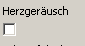
\includegraphics[width=2.2cm]{images/boolfield.png}
\end{center}
\subsubsection{Attribute}
\begin{description}
    \item[default:] Standardwert, wenn die Messung neu erfasst wird (nur
                    \texttt{true} oder \texttt{false} werden akzeptiert)
\end{description}
\subsubsection{Beispiel}
\begin{lstlisting}
<boolfield name="herger" title="Herzgeraeusch" />
\end{lstlisting}

\subsection{datafield}
Verweis auf andere Messungen
\begin{center}
    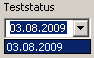
\includegraphics[width=2.6cm]{images/datafield.png}
\end{center}
\subsubsection{Attribute}
\begin{description}
    \item[type:] Name des Messungstyps auf den verwiesen werden soll
\end{description}
\subsubsection{Beispiel}
\begin{lstlisting}
<datafield  name="vorekg" title="Vorekg" type="ekg" />
\end{lstlisting}

\subsection{calcfield}
Errechnetes Feld
\begin{center}
    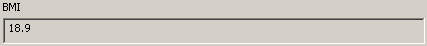
\includegraphics[width=12cm]{images/calcfield.png}
\end{center}
\subsubsection{Attribute}
\begin{description}
    \item[places:] Anzahl der Nachkommastellen beim Ergebnis
    \item [formatpattern:] Pattern für die Formatierung der angezeigten Zahl \textit{[Standard: \#0.\#]}\\
    Siehe auch Beschreibung bei numfield.
    \item [roundingmode:] Modus wie die angezeigte Zahl gerundet wird \textit{[Standard: HALF\_UP]}\\
    Siehe auch Beschreibung bei numfield.
\end{description}
\subsubsection{Unterelemente}
Beim calcfield sind 2 verschiedene Unterelemente vorgesehen. Zum einen ist das
\texttt{var}, das es ermöglicht, Felder aus der Messung als Variablen in die
Formel zu importieren, zum andern \texttt{formula}, das die eigentliche Formel
enthält.\\
\\
Bei \texttt{var} müssen 2 Attribute angegeben werden \texttt{name}, der
Name wie die Variable in der Formel heissen soll, und \texttt{source} mit dem
Feldnamen in der Messung. Bei Datenfeldern kann beispielsweise mit
\texttt{datenfeldname.gewicht} auf das Feld \texttt{gewicht} in der
re\-fe\-ren\-zier\-ten Messung zugegriffen werden. Das Ganze kann beliebig tief
verschachtelt werden.\\
\\
Beim Element \texttt{formula} muss mit dem Attribut \texttt{interpreter} der zu
benutzende Interpreter ausgewählt werden. Im Moment steht jedoch nur «beanshell»
zur Verfügung.
\subsubsection{Beispiel}
\begin{lstlisting}
<calcfield name="bmi" title="BMI" places="2">
  <var name="gewicht" source="gewicht" />
  <var name="groesse" source="groesse" />
  <formula interpreter="beanshell">
    return gewicht/(groesse*groesse);
  </formula>
</calcfield>
\end{lstlisting}
\subsection{datefield}
Auswahlfeld für ein Datum
\begin{center}
    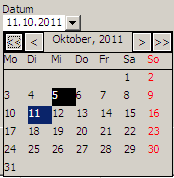
\includegraphics[width=4.6cm]{images/datefield.png}
\end{center}
\subsubsection{Beispiel}
\begin{lstlisting}
<datefield name="erfdatum" title="Datum" />
\end{lstlisting}
\subsection{counterfield}
Automatisch generierte Laufnummer für die Messung
\begin{center}
    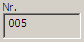
\includegraphics[width=2.2cm]{images/counterfield.png}
\end{center}

\subsubsection{Attribute}
\begin{description}
    \item[countermode:] Modus für den Zähler \textit{[Standard: global\_counter]}\\
    Derzeit sind keine weiteren Modi implementiert.
    \item[startvalue:] Startwert für den Zähler \textit{[Standard: 0]}
    \item [formatpattern:] Pattern für die Formatierung der angezeigten Zahl  \textit{[Standard: \#,000]}\\
    Siehe auch Beschreibung bei numfield.
    \item [roundingmode:] Modus wie die angezeigte Zahl gerundet wird \textit{[Standard: HALF\_UP]}\\
    Siehe auch Beschreibung bei numfield.
\end{description}

\subsubsection{Beispiel}
\begin{lstlisting}
<counterfield name="number" title="Nr." countermode="global_counter"
startvalue="0" formatpattern="#,000" />
\end{lstlisting}
\section{IDataAccess-Schnittstelle}
Das \texttt{hilotec-messwerte}-Plugin stellt die IDataAccess-Schnittstelle, die
auch von an\-de\-ren Elexis-Plugins benutzt wird, zur Verfügung. Damit wird es unter
anderem auch möglich in Briefen und Berichten auf Werte aus erfassten Messungen
zurückzugreifen. Allgemeine Informationen zu dieser Schnittstelle sind dem
Elexis-Handbuch zu ent\-neh\-men, wo die Schnittstelle genauer beschrieben wird. Im
Folgenden soll nur auf den plug\-in\-spe\-zi\-fi\-schen Teil eingegangen werden.

Das Plugin benutzt den Identifier \texttt{Messwerte} fuer die Schnittstelle. Das
heisst, die Platzhalter für den Zugriff haben die Form
\texttt{Messwerte:Patient:auswahl:daten}. Wobei für den Teil \texttt{auswahl} die
folgenden Möglichkeiten bestehen:
\begin{description}
    \item[\texttt{dd.mm.yyyy}:] Messung von genau dem angegebenen Datum
    \item[first:] Erste Messung des Patienten
    \item[last:] Letzte Messnug des Patienten
    \item[firstsince=\texttt{dd.mm.yyyy}:] Erste Messung nach dem angegebenen
                                           Datum
    \item[lastbefore=\texttt{dd.mm.yyyy}:] Letzte Messung vor dem angegebenen
                                           Datum
\end{description}

Der Teil \texttt{daten} hat die Form \texttt{typ.feld}, wobei \texttt{typ} den
Namen des Messungstyp bezeichnet, und \texttt{feld} den Namen des Feldes in dem
Typ. Kommen Datenfelder vor, kann mit einem weiteren Punkt der Feldname in der
referenzierten Messung spezifiziert werden. Auch hier können die Datafelder
wieder beliebig verschachtelt werden.

\subsubsection{Beispiel}
\begin{lstlisting}
[Messwerte:Patient:last:status.gewicht]
\end{lstlisting}


\section{Layout Steuerung}
Standardmässig wird bei Doppelklick auf eine Messwertreihe ein Dialogfenster
geöffnet, welches alle Werte untereinander zum Eingeben und Ändern anbietet. Auf
Wunsch kann den einzelnen Messwertreihen aber auch Darstellungsinformation
mitgegeben werden. Dies wird gemacht, indem man ein Element $<$design$>$ der
$<$datatype$>$ - Definition zufügt.

\section{Beispiel messwerte\_v2.xml}
\begin{lstlisting}
<?xml version="1.0"?>
<datatypes>
  <datatype name="status" title="Status">
    <numfield name="groesse" title="Grösse" unit="m" default="1.70" />
    <numfield name="gewicht" title="Gewicht" unit="kg" />
    <calcfield name="bmi" title="BMI" places="2">
      <var name="gewicht" source="gewicht" />
      <var name="groesse" source="groesse" />
      <formula interpreter="beanshell">
        return Math.round(gewicht/(groesse*groesse)*10)/10.0;
      </formula>
    </calcfield>
    <design>
      <panel type="grid">
        <attribute name="columns" value="1" />
        <panel type="display">
          <attribute name="url" value="http://www.elexis.ch" />
          <attribute name="size" value="600,150" />
        </panel>
        <panel type="grid">
          <attribute name="columns" value="3" />
          <panel type="field">
            <attribute name="ref" value="groesse" />
            <attribute name="validpattern" value="[0-9\\.]*" />
            <attribute name="invalidmessage"
            value="Es sind nur Zahlen und der Dezimalpunkt zulässig" />
          </panel>
          <panel type="field">
            <attribute name="ref" value="gewicht" />
            <attribute name="validpattern" value="[0-9\\.]*" />
            <attribute name="invalidmessage"
            value="Es sind nur Zahlen und der Dezimalpunkt zulässig" />
          </panel>
          <panel type="field">
            <attribute name="ref" value="bmi" />
          </panel>
        </panel>
      </panel>
    </design>
  </datatype>

  <datatype name="ident_basis" title="Identifikation und Basisinfo">
    <counterfield name="number" title="Nr." countermode="global_counter"
                  formatpattern="#,000" />
    <strfield name="erheber" title="Erheberin" />
    <numfield name="idpat" title="ID Pat" formatpattern="#0000" />
    <calcfield name="patname" title="Name">
      <formula interpreter="beanshell">
        return actPatient.getName() + " " + actPatient.getVorname();
      </formula>
    </calcfield>
    <design>
      <panel type="grid">
        <attribute name="columns" value="1" />
        <panel type="display">
          <attribute name="url" value="http://www.elexis.ch" />
          <attribute name="size" value="600,150" />
        </panel>
        <panel type="grid">
          <attribute name="columns" value="2" />
          <panel type="field">
            <attribute name="ref" value="number" />
          </panel>
          <panel type="field">
            <attribute name="ref" value="erheber" />
          </panel>
          <panel type="field">
            <attribute name="ref" value="idpat" />
            <attribute name="validpattern" value="[0-9][0-9][0-9][0-9]" />
            <attribute name="invalidmessage" 
              value="Es ist nur eine vierstellige ganze Zahl zulässig" />
          </panel>
          <panel type="field">
            <attribute name="ref" value="patname" />
          </panel>
        </panel>
      </panel>
    </design>
  </datatype>
</datatypes>
\end{lstlisting}

\end{document}
